\documentclass{article}
\usepackage[utf8]{inputenc}
\usepackage{graphicx}
\usepackage{multirow}
\usepackage{float}
\usepackage{indentfirst}
\usepackage{appendix}
\usepackage{listings}

% For Adding MATLAB code as .m file
\usepackage{color} %red, green, blue, yellow, cyan, magenta, black, white
\definecolor{mygreen}{RGB}{28,172,0} % color values Red, Green, Blue
\definecolor{mylilas}{RGB}{170,55,241}

\graphicspath{ {./images/} }

\title{Speech Recognition through Mel Frequency Cepstral Coefficients and Dynamic Time Warping}
\author{Thomas Smallarz}
\date{13 December 2020}

\begin{document}

% For adding MATLAB code in appendix
\lstset{language=Matlab,%
    %basicstyle=\color{red},
    breaklines=true,%
    morekeywords={matlab2tikz},
    keywordstyle=\color{blue},%
    morekeywords=[2]{1}, keywordstyle=[2]{\color{black}},
    identifierstyle=\color{black},%
    stringstyle=\color{mylilas},
    commentstyle=\color{mygreen},%
    showstringspaces=false,%without this there will be a symbol in the places where there is a space
    numbers=left,%
    numberstyle={\tiny \color{black}},% size of the numbers
    numbersep=9pt, % this defines how far the numbers are from the text
    emph=[1]{for,end,break},emphstyle=[1]\color{red}, %some words to emphasise
    %emph=[2]{word1,word2}, emphstyle=[2]{style},    
}

\maketitle
\tableofcontents

\section*{Introduction}
Speech is a fundamental mode of communication between people, even in this age of non-verbal communication (email, text, etc.), so the benefits of being able to translate human speech to a digital format is obvious. 

This report will explain implementing a method of speech recognition in MATLAB R2020b using Mel Frequency Cepstral Coefficients and Dynamic Time Warping with the intention of implementing this method on a low-cost embedded target.

\section{Method}
Most modern automatic speech recognition (ASR) systems have the same structure. It is as follows:
\begin{enumerate}
    \item Speech is recorded and digitized
    \item Features of waveform are extracted
    \item Strings of phonemes are recognized based on features
    \item Words and strings of words are assembled based on language models
\end{enumerate}

\begin{figure}[H]
    \centering
    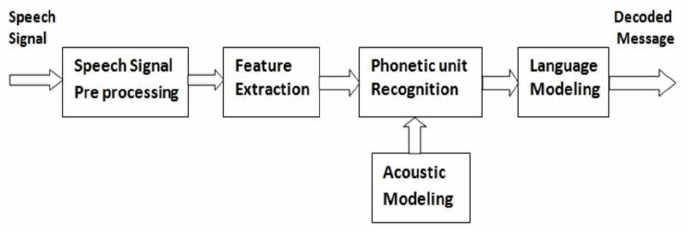
\includegraphics[width=\linewidth]{blockdiagram.png}
    \caption{General speech recognition system diagram}
    \label{fig:diagram}
\end{figure}

As of now, we won't concern ourselves with the first step -- recording and digitizing audio. This will be talked about a little in the Implementation section later on. Also, language modeling will not be discussed in this report.
% **************************
% *** BEGIN MFCC SECTION ***
% **************************
\subsection{Mel Frequency Cepstral Coefficients}
Before using algorithms to determine the likelihood of speech utterances to be specific words, the data is typically manipulated to gain characteristics that describe what is being said.

In this implementation Mel Frequency Cepstral Coefficients (MFCC) are used. There are numerous ways to extract features or characteristics of speech. This is one method that is used.

\subsubsection{Cepstral}
To understand how to derive coefficients of the MFC, it is first important to learn what the "cepstrum" is. The cepstrum of a signal is the result of taking the inverse Fourier transform (IFT) of the logarithm of the Fourier transform (FT) of a signal. Or,

\begin{center}
$|\mathcal{F}^{-1}\{\log|(\mathcal{F}\{x[n]\})^{2}|\}|^{2}$    
\end{center}

\subsubsection{Mel Scale}
The Mel scale is a scale based on the perceptions of human hearing. It is a mapping function that separates pitches by what humans consider to be equal distance. A common formula to convert frequency from hertz into mels is:

\begin{center}
    $m=2595log_{10}(1+f/700)$
\end{center}

\begin{figure}[H]
    \centering
    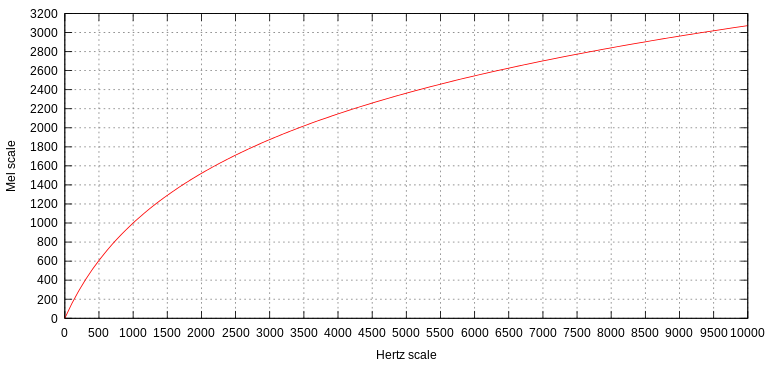
\includegraphics[width=\linewidth]{melscale.png}
    \caption{Mel scale vs. hertz}
    \label{fig:melscale}
\end{figure}

\subsubsection{Mel Frequency Cepstral}
Including both these concepts, the difference between Cepstral and Mel Frequency Cepstral is that MFC has its initial spectrum mapped to the mel scale before taking the logarithm. The common derivation of MFCC's is as follows:

\begin{enumerate}
    \item Take the Fourier Transform of signal
    \item Find the powers of that spectrum
    \item Map onto the mel scale (typically with triangle filters)
    \item Take the logs at each mel frequency
    \item Take the discrete cosine transform (DCT) of the mel log powers
\end{enumerate}
\noindent
Then, the MFC coefficients are the amplitudes of the resulting spectrum.

% *************************
% *** BEGIN DTW SECTION ***
% *************************
\subsection{Dynamic Time Warping}
Dynamic Time Warping (DTW) is an algorithm that measures the similarity between two sequences in time (or other dependent variable) that may vary in speed. It calculates a distance matrix, then the shortest weighted path of that matrix is the "distance" sequence used to map one of the signals onto the other. So, with $A_i$ and $B_i$ sequences

\begin{enumerate}
    \item Create distance matrix of size i x j
    \item Find shortest weighted distance from opposite corners of distance matrix
\end{enumerate}

\begin{figure}[H]
    \centering
    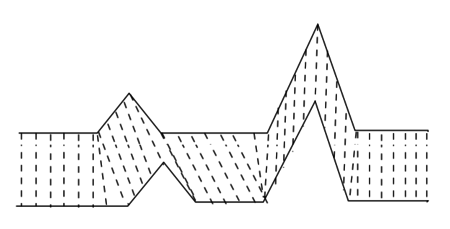
\includegraphics[width=\linewidth]{dtw_image.png}
    \caption{Example of mapping one sequence onto another using DTW}
    \label{fig:dtw_map}
\end{figure}

\subsubsection{Creating distance matrix}
Creating the distance matrix is done with a simple equation. If the values of $A_i$ and $B_j$ are put on row and column side of the matrix respectively, then the values at $D_{i,j}$ are:
\begin{center}
    $D(i,j) = |B_j - A_i| + min(D(i-1,j-1),D(i-1,j),D(i,j-1))$
\end{center}
\noindent
This is calculated starting at the first place in the sequence ($D_{0,0}$) and working towards the last place ($D_{i,j}$). Values $D(i-1,j-1)$, $D(i-1,j)$, and $D(i,j-1)$ are used when they have been already computed.

There are more computationally simpler methods of computing this distance matrix, but in short, this is how it is calculated.

\subsubsection{Finding shortest path}
Once a distance matrix is created we need to find the values to warp the two sequences by to to align them. These values are found by starting in the upper corner of the distance matrix ($D(i,j)$) and recursively find the minimum of $D(i-1,j-1)$, $D(i-1,j)$, and $D(i,j-1)$ until reaching the lower corner ($D(i,j)$). 

The amplitude values of the distance matrix could be likened to the height of a mountain range, and the path you take to the origin is the valley between the mountain peaks.

\section{Implementation}
Now, armed with the means to find the MFCC's and perform a DTW. We can create some training data (multiple recordings of some word) and have an input and see if our system can recognized the inputted word.

\subsection{Digitizing Audio}
First is to record the audio. In MATLAB there is a audiorecorder( ) function that uses your default system microphone and has parameters: sampling frequency, bit size to store data in, and number of channels to record.

\begin{itemize}
    \item Sampling Frequency: A quick Google search brings us to the Voice Frequency Wikipedia page that says a sampling rate of 8,000Hz is sufficient (a 4000Hz bandwidth doubled)
    \item Bit Size: Let's go with 16-bit Integers for now. Implementing on lower-cost hardware may require less size
    \item Number of Channels: One channel for one microphone
\end{itemize}

\begin{figure}[H]
    \centering
    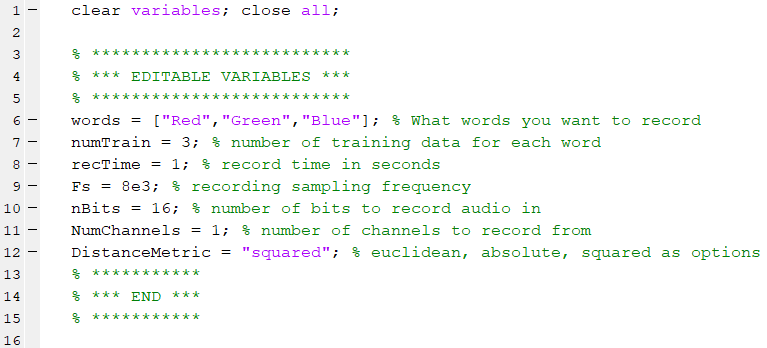
\includegraphics[width=\linewidth]{MATLAB_variables.png}
    \caption{}
    \label{fig:MATLAB_variables}
\end{figure}

Now, we create an instance of the audiorecorder and record each word "numTrain" times with a one second duration to record.

\begin{figure}[H]
    \centering
    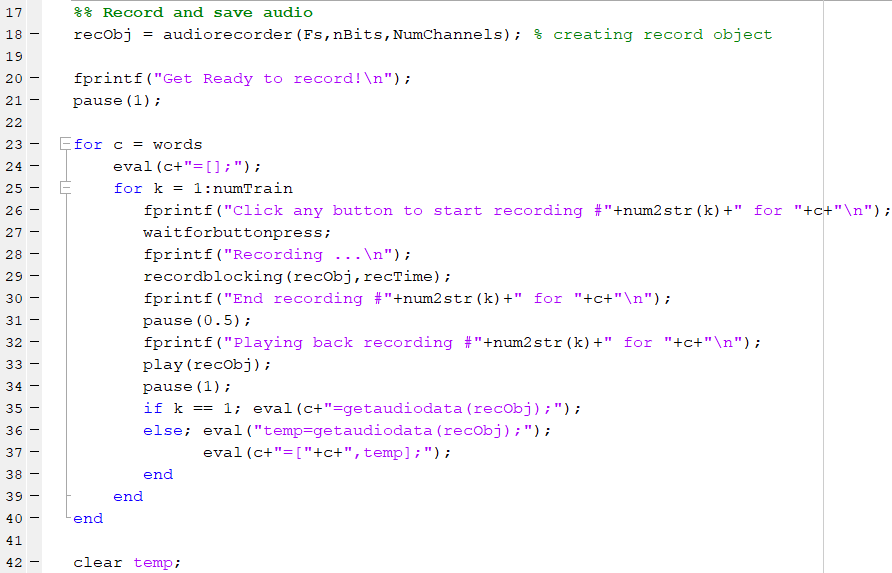
\includegraphics[width=\linewidth]{MATLAB_recordTrainingAudio.png}
    \caption{}
    \label{fig:MATLAB_recTrainAudio}
\end{figure}

After this we can record our input audio using the same method.

\begin{figure}[H]
    \centering
    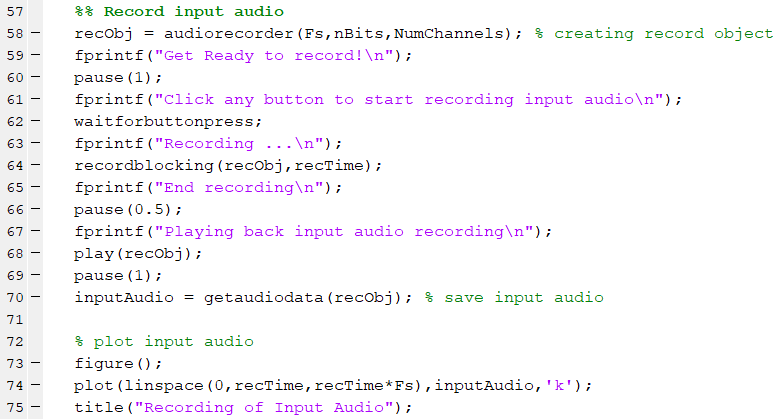
\includegraphics[width=\linewidth]{MATLAB_inputaudio.png}
    \caption{}
    \label{fig:MATLAB_inputAudio}
\end{figure}

Plotting recorded audio:
\begin{figure}[H]
    \centering
    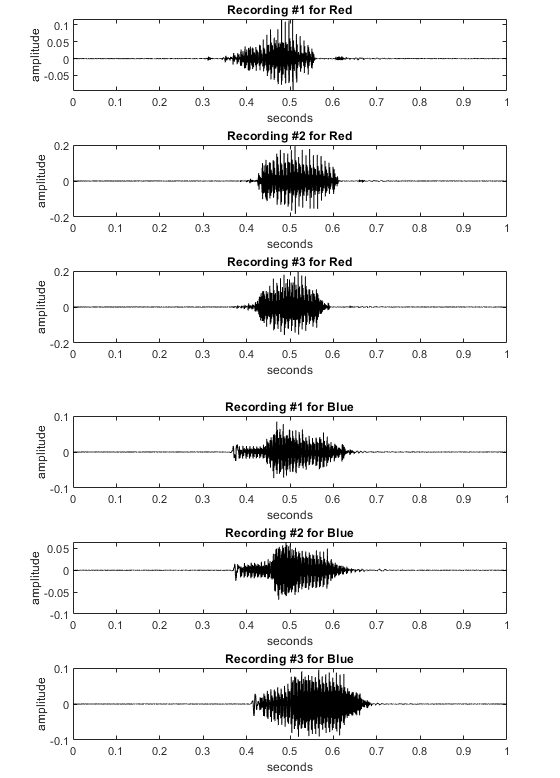
\includegraphics[width=\linewidth]{REC_RB.png}
    \caption{"Red" and "Blue" recorded audios}
    \label{fig:MATLAB_REDandBLUE}
\end{figure}

\begin{figure}[H]
    \centering
    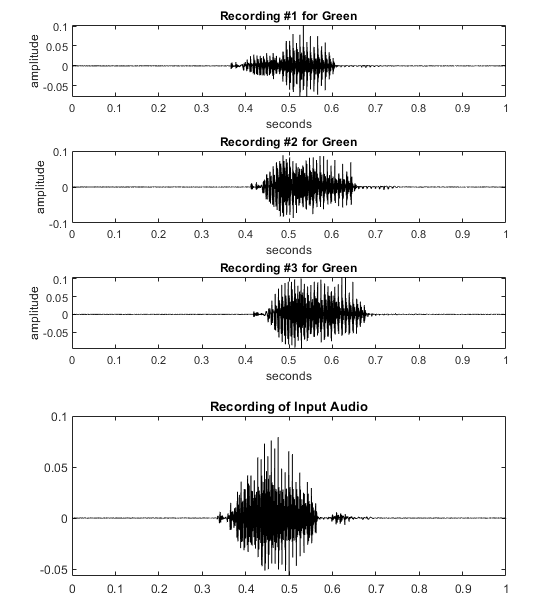
\includegraphics[width=\linewidth]{REC_GIN.png}
    \caption{"Green" and input recorded audios}
    \label{fig:MATLAB_GREENandINPUT}
\end{figure}

Now that we have all our "training" audio and input audio saved it's time to calculate our MFC coefficients.

\subsection{Feature Extraction}
Using the MFCC method we talked about earlier, we can use the built-in mfcc( ) MATLAB function. This function has input parameters for the audio amplitude values, and sampling frequency, and returns the mel frequency cepstral coefficients. The algorithm from MATLAB's documentation for this function is:

\begin{figure}[H]
    \centering
    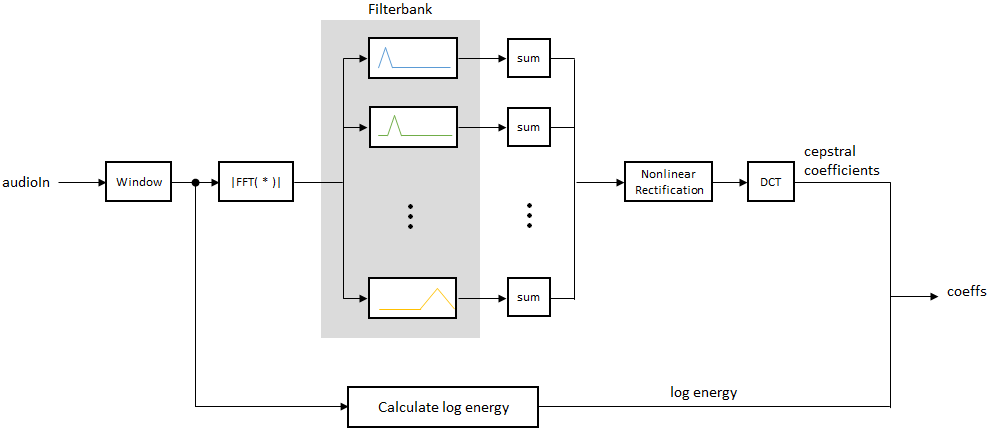
\includegraphics[width=\linewidth]{MATLAB_mfcc.png}
    \caption{}
    \label{fig:MATLAB_mfcc}
\end{figure}

This is implemented in MATLAB as:

\begin{figure}[H]
    \centering
    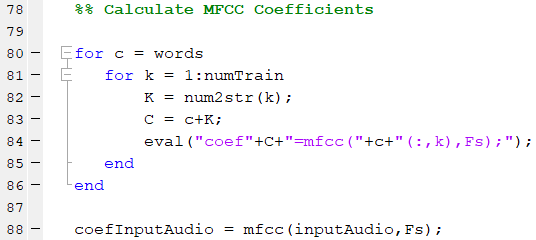
\includegraphics[width=\linewidth]{MATLAB_mfcc2.png}
    \caption{}
    \label{fig:MATLAB_mfcc2}
\end{figure}

\subsection{Feature Recognition}
Now that we've calculated the MFC coefficients for each audio sequence we can compare the inputted audio against the templates using dynamic time warping to see which template has the lowest distance when compared to our inputted audio.

For this, MATLAB has a built-in dtw( ) function that has input parameters of an input vector "x" and an input vector "y". The order of inputting "x" and "y" does not matter. This function outputs: the total calculated euclidean distance of "x" and "y", the warping path for "x", and the warping path for "y".

\begin{figure}[H]
    \centering
    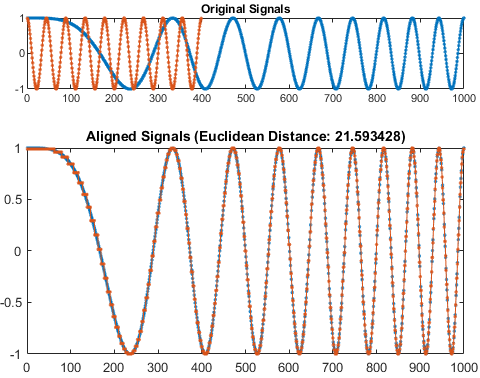
\includegraphics[width=\linewidth]{dtw_docu.png}
    \caption{Example of how dtw( ) "maps" one sequence to another}
    \label{fig:MATLAB_dtw_docu}
\end{figure}

Implementing this in MATLAB:

\begin{figure}[H]
    \centering
    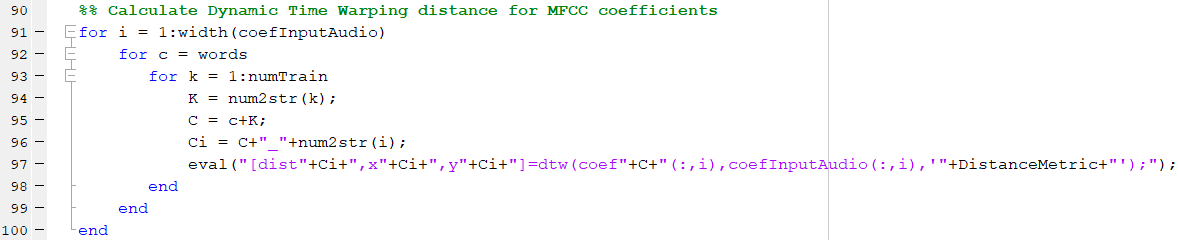
\includegraphics[width=\linewidth]{MATLAB_dtw.png}
    \caption{}
    \label{fig:MATLAB_dtw}
\end{figure}

Then plotting results gives us:

\begin{figure}[H]
    \centering
    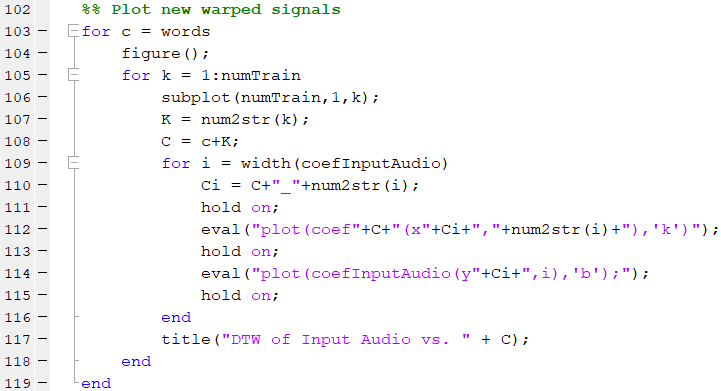
\includegraphics[width=\linewidth]{MATLAB_plotwarped.png}
    \caption{}
    \label{fig:MATLAB_plotwarped}
\end{figure}

\begin{figure}[H]
    \centering
    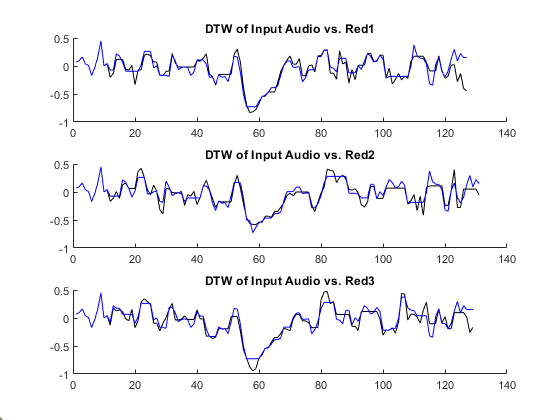
\includegraphics[width=\linewidth]{DTWMFCC_R.png}
    \caption{DTW of Input vs. Red MFC Coefficients}
    \label{fig:MATLAB_dtwR}
\end{figure}

\begin{figure}[H]
    \centering
    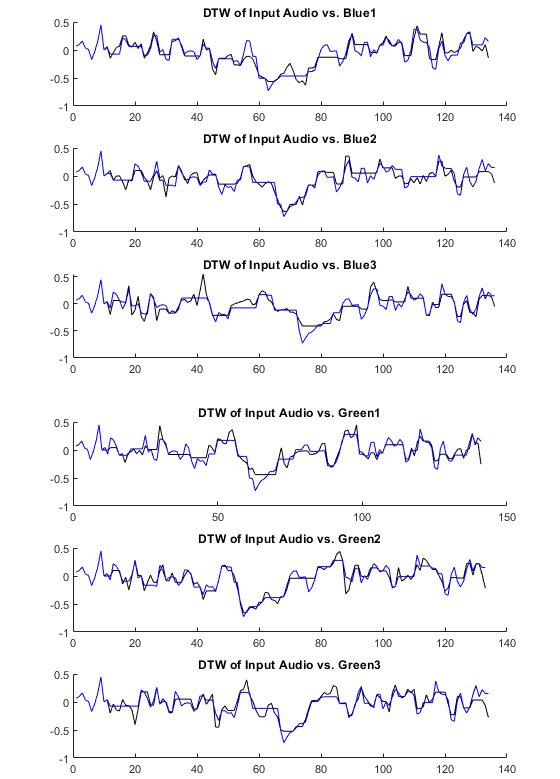
\includegraphics[width=\linewidth]{DTWMFCC_BG.png}
    \caption{DTW of Input vs. Blue/Green MFC Coefficients}
    \label{fig:MATLAB_dtwBG}
\end{figure}

Then, summing all the distances from the Red, Blue, and Green coefficient matrices gives us:

\begin{figure}[H]
    \centering
    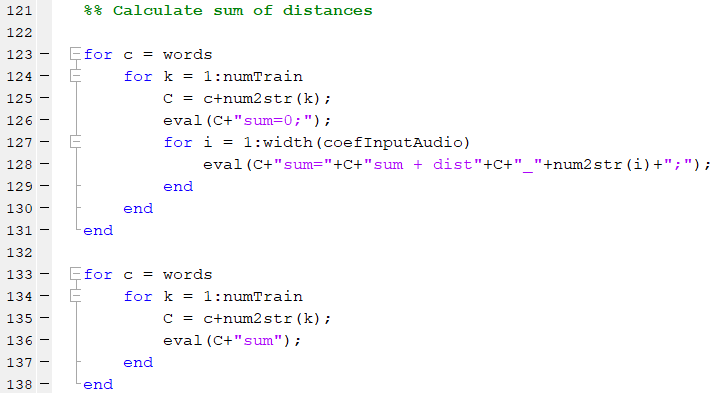
\includegraphics[width=\linewidth]{MATLAB_sumofdist.png}
    \caption{}
    \label{fig:MATLAB_sumofdist}
\end{figure}

Summing each gives us:
\begin{center}
    \begin{tabular}{c c c}
    \hline
    Color & Set & Distance \\
    \hline
    \multirow{3}{4em}{Red} & 1 & 95.78 \\
    & 2 & 180.09\\
    & 3 & 139.43\\
    \hline
    \multirow{3}{4em}{Blue} & 1 & 179.83 \\
    & 2 & 172.95\\
    & 3 & 292.08\\
    \hline
    \multirow{3}{4em}{Green} & 1 & 208.80 \\
    & 2 & 241.63\\
    & 3 & 201.73\\
    \hline
    \end{tabular}
\end{center}

From this we can see that training sets from the color red have the lowest two distances. This is a good thing because in this case I did say "Red" for my input recording.

\appendix
\section{MATLAB}

\lstinputlisting{run_mfcc.m}
\newpage
\section*{References}
\begin{enumerate}
    \item Bhadragiri, J.M., and Ramesh, B.N., \emph{Speech Recognition using MFCC and DTW}, VIT University, Vellore, India, 2014
    \item Kare, C.B., and Navale, V.S., \emph{Speech recognition by Dynamic Time Warping}, IOSR Journal of Electronics and Communication Engineering, Pune, 2015
    \item Kesarkar, M.P., \emph{Feature Extraction for Speech Recognition}, IIT Bombay, Mumbai, India, 2003
    \item Narang, S., and Gupta, D., \emph{Speech Feature Extraction Techniques: A Review}, Amity University, Noida, India, 2015
    \item Rao, K.S., and Manjunath K.E., \emph{Speech Recognition Using Articulatory and Excitation Source Features}, 2017
\end{enumerate}

\end{document}
